\documentclass[11pt, a4paper]{book}

\usepackage{mathpazo}
\usepackage[utf8]{inputenc}
\usepackage[T1]{fontenc}
\usepackage{amsmath}
\usepackage{amsfonts}
\usepackage{amssymb}
\usepackage{amsthm}
\usepackage[colorlinks=true, pagebackref=true]{hyperref}
\usepackage[alphabetic]{amsrefs}
\usepackage{mathtools}
\usepackage{xcolor}
\usepackage{titlesec} %reasonable chapter headings
\usepackage{stmaryrd} %double brackets
\usepackage{tikz}
\usetikzlibrary{arrows,positioning,through}

\usepackage{chngcntr}
\counterwithout{equation}{section} %this fixes equation numbering

\titleformat{\chapter}[display]
  {\normalfont\bfseries}{}{0pt}{\Huge} %this eliminates the 'Chapter n' heading

\hypersetup{linkcolor=teal, citecolor=teal}

\newcommand{\NN}{\mathbb{N}}
\newcommand{\ZZ}{\mathbb{Z}}
\newcommand{\QQ}{\mathbb{Q}}
\newcommand{\RR}{\mathbb{R}}
\newcommand{\CC}{\mathbb{C}}

\newcommand{\kQ}{k\langle Q\rangle}
\newcommand{\KQ}{k\langle\langle Q\rangle\rangle}
\newcommand{\cyc}{\mathrm{cyc}}

\theoremstyle{plain}
\newtheorem{prop}{Proposition}[chapter]
\theoremstyle{definition}
\newtheorem{exmp}[prop]{Example}

\begin{document}

\begin{chapter}{Preliminaries}
Throughout the text, $k$ will denote a field of characteristic zero.
\begin{section}{The path algebra of a quiver}
A \emph{quiver} is a quadruple $Q=(Q_0, Q_1, s,t)$, where $Q_0$ and $Q_1$ are finite sets whose elements are called \emph{vertices} and \emph{arrows} respectively, and $s,t:Q_1\to Q_0$ are functions that associate to each arrow $\alpha\in Q_1$ its \emph{source} $s(\alpha)\in Q_0$ and its \emph{target} 
$t(\alpha)\in Q_0$. We will usually abbreviate the fact that an arrow $\alpha\in Q_1$ has source $a$ and target $b$ using the notation $\alpha:a\to b$. We will also omit mentioning $s$ and $t$ explicitly when they are clear from context.

One can represent a quiver graphically as an oriented graph allowing loops and multiple arrows between the same pair of vertices. The following are some examples of quivers:
\[
\begin{tikzpicture}[->, node distance=1cm, thick, auto]
\tikzstyle{every node} = [circle, fill=gray!30, minimum size=.5cm]
\tikzset{every loop/.style={looseness=15}}
\node (a) at (0:1) {};
\node (b) at (120:1) {};
\node (c) at (240:1) {};
\path (a) edge [bend right] (b)
(b) edge [bend right] (c)
(c) edge [bend right] (a)
(a) edge [in=15, out=-15, loop] (a)
(b) edge [in=135, out=105, loop] (b)
(c) edge [in=255, out=225, loop] (c);
\node (d) [right=of a,xshift=2cm] {};
\node (e) [right=of d] {};
\foreach \from/\to in {d/e, e/d}
\draw (d.40) -- (e.140);
\draw (e) -- (d);
\draw (d.320) -- (e.220);
\end{tikzpicture}
\]
\[
\begin{tikzpicture}[->,node distance=1cm, thick]
\tikzstyle{every node} = [circle, fill=gray!30, minimum size=.5cm]
\node (1) {};
\node (2) [right=of 1] {};
\node (3) [right=of 2] {};
\node (4) [right=of 3] {};
\node (5) [right=of 4] {};
\node (6) [right=of 5] {};
\node (7) [right=of 6] {};
\node (8) [below=of 3] {};
\foreach \from/\to in {2/1, 3/2, 3/4, 3/8, 4/5, 5/6, 6/7}
\draw [->] (\from) -- (\to);
\end{tikzpicture}
\]
Let $Q=(Q_0, Q_1, s, t)$ be a quiver and consider the $k$-vector spaces $R=k^{Q_0}$ and $A=k^{Q_1}$, which we will call the \emph{vertex span} and \emph{arrow span} of $Q$, respectively. The space $R$ is a commutative $k$-algebra with the product given by pointwise multiplication. Thus, we can consider an $R$-bimodule structure on $A$ given as follows: if $r\in Q_0$, $\alpha\in Q_1$ then we define $r\alpha = \delta_{r,t(\alpha)} \alpha$ and analogously $\alpha r = \delta_{r, s(\alpha)}\alpha$, and extend the action linearly. Therefore, a vertex $r$ acts as the identity on the left (right) of an arrow $\alpha$ if the target (source) of $\alpha$ is $r$, and otherwise acts as zero. The \emph{path algebra} $\kQ$ associated to the quiver $Q$ is the graded tensor algebra
\[
\kQ = \bigoplus_{n=0}^\infty A^{\otimes_R n},
\]
where we set $A^{\otimes_R 0}=R$. For the sake of simplicity we will usually notate $A^{\otimes_R n}$ as $A^n$ and an elementary tensor $\alpha_n\otimes\dots\otimes \alpha_1$ as $\alpha_n\dots\alpha_1$. Notice that a non-zero element of the form $\alpha_n\dots\alpha_1$ consists of a sequence of \emph{concatenable} arrows $\alpha_i$, that is, arrows such that $s(\alpha_{i+1})=t(\alpha_i)$. We will call such an element a \emph{path of length n}. It is worth observing that the collection of all paths of length $n$ form a basis of $A^n$ as a $k$-vector space. Since $Q_0$ is a basis of $A^0=R$, we will refer to elements of $Q_0$ as \emph{paths of length 0}, which we will usually call \emph{trivial} or \emph{stationary} paths. Considering $Q_0$ and $Q_1$ are in bijection with paths of length 0 and 1 respectively, we will denote the set of paths of length $n$ as $Q_n$ and the set of all paths as $Q_*$. We can now define source and target functions $s,t:Q_*\to Q_0$ as follows: if $u=\alpha_n\dots\alpha_0\in Q_n$ with $n>0$, then $s(u)=s(\alpha_0)$ and $t(u)=t(\alpha_n)$. Otherwise, if $u=r\in Q_0$ then $s(u)=t(u)=r$. Thus, one easily checks that if $a,b\in Q_0$, the space spanned by paths with source $a$ and target $b$ is exactly $b\kQ a$.

The path algebra satisfies the following useful universal property:

\begin{prop} Let $Q$ be a quiver and $\Lambda$ be an associative $k$-algebra with unit. Suppose $f_0:Q_0\to \Lambda$, $f_1:Q_1\to\Lambda$ are maps satisfying:
\begin{enumerate}
\item $\sum_{r\in Q_0} f_0(r)=1$.
\item If $a\in Q_0$, then $f_0^2(a)=f_0(a)$.
\item If $a\neq b\in Q_0$, then $f_0(a)f_0(b)=0$.
\item If $\alpha:a\to b$ is an arrow in $Q_1$, then $f_1(\alpha) = f_0(b) f_1(\alpha) f_0(a)$.
\end{enumerate}
Then, there exists a unique $k$-algebra morphism $f:\kQ\to \Lambda$ extending $f_0$ and $f_1$.
\end{prop}
\begin{proof} If $n\geq 1$, define $f(\alpha_n\dots\alpha_1)=f_1(\alpha_n)\dots f_1(\alpha_0)$ and let $f(r)=f_0(r)$ for $r\in Q_0$. As the set of all paths forms a basis of $\kQ$ as a vector space, this defines a $k$-linear map $f:\kQ\to \Lambda$. Condition 1 guarantees that such a map preserves the unit and conditions 2, 3 and 4 guarantee that it preserves products involving stationary paths. Since by definition $f$ preserves products of non-trivial paths, we conclude that $f$ is a $k$-algebra morphism extending $f_0$ and $f_1$. As for uniqueness, consider another extension $g:\kQ\to\Lambda$. Since $g$ is a $k$-algebra morphism, we have that $g(\alpha_n\dots\alpha_1)= g(\alpha_n)\dots g(\alpha_1)= f_1(\alpha_n)\dots f_1(\alpha_1)=f(\alpha_n\dots\alpha_1)$ for $n\geq 1$ and $g(r)=f_0(r)=f(r)$ for all $r\in Q_0$. Thus $g$ agrees with $f$ in a basis, and so $g=f$ as wanted.
\end{proof}
Let us now consider some examples:
\begin{exmp} Let $Q$ be the quiver with vertices $\{1,\dots,n\}$ and no arrows:
\[
\begin{tikzpicture}[node distance=1cm, auto, thick]
\tikzstyle{every node} = [circle, fill=gray!30, minimum size=.5cm, inner sep=.07cm]
\node (1) {1};
\node (2) [right=of 1] {2};
\node (3) [right=of 2] {3};
\node (4) [right=of 3, fill=white] {...};
\node (5) [right=of 4] {n};
\end{tikzpicture}
\]
The path algebra $\kQ$ is then isomorphic to $k^n = ke_1\oplus\dots\oplus ke_n$, where multiplication is given by $e_i e_j = \delta_{i,j} e_i$ and extended linearly.
\end{exmp}

\begin{exmp}\label{one-loop} Let $Q$ be the quiver with a single vertex $1$ and a single arrow $\alpha:1\to 1$:
\[
\begin{tikzpicture}[->, thick]
\tikzset{every loop/.style={looseness=15}}
\node[circle, fill=gray!30, minimum size=.5cm, inner sep=.07cm]  (1) {1};
\path (1) edge [loop above] node {$\alpha$} (1);
\end{tikzpicture}
\]
The path algebra $\kQ$ has a basis given by $\{e_a, \alpha, \alpha^2, \dots\}$. It is easily seen that $\kQ$ is isomorphic to the polynomial algebra $k[x]$, via the map sending $\alpha \mapsto x$ and $1\mapsto 1$.
\end{exmp}
\begin{exmp}\label{several-loops} More generally, let $Q$ be the quiver with a single vertex $1$ and $n$ arrows $\alpha_n:1\to 1$:
\[
\begin{tikzpicture}[->, auto, thick]
\tikzset{every loop/.style={looseness=15}}
\node[circle, fill=gray!30, minimum size=.5cm, inner sep=.07cm]  (1) {1};
\node[circle, fill=white] (2) at +(270: 1) {...};
\path (1) edge [loop left] node {$\alpha_5$} (1);
\path (1) edge [loop above] node {$\alpha_3$} (1);
\path (1) edge [loop right] node {$\alpha_1$} (1);
\path (1) edge [in=30, out=60, loop] node {$\alpha_2$} (1);
\path (1) edge [in=210, out=240, loop] node {$\alpha_6$} (1);
\path (1) edge [in=120, out=150, loop] node {$\alpha_4$} (1);
\path (1) edge [in=300, out=330, loop] node {$\alpha_n$} (1);
\end{tikzpicture}
\]
Then, the path algebra $\kQ$ is isomorphic to the free algebra on $n$ generators $k\langle x_1,\dots, x_n\rangle$, via the map sending $\alpha_i\mapsto x_i$ and $1\mapsto 1$.
\end{exmp}

A path $u\in Q_n$ with $n>1$ such that $s(u)=t(u)$ is called a \emph{cycle}, and a quiver containing no cycles is said to be \emph{acyclic}. As we can infer from the previous examples, the existence of cycles in the quiver is closely related to the dimension of the path algebra. More precisely, we have:

\begin{prop}\label{acyclic-fin-dim}
Let $Q$ be a quiver and $\kQ$ its associated path algebra. Then $\kQ$ is finite-dimensional iff $Q$ is acyclic.
\end{prop}
\begin{proof} Suppose $\kQ$ is infinite-dimensional. Then the set of all paths $Q_*$, which is a basis for $\kQ$, must be infinite. Since the quiver has only a finite number of arrows, there's only a finite number of paths of less than a fixed length. Therefore, if the set of paths $Q_*$ is infinite, then there exist arbitrarily long paths. Let $n$ be the number of vertices in $Q_0$ and pick a path $\alpha_m\dots\alpha_1$ with $m>n$. Then $s(\alpha_i) = t(\alpha_j)$ for some $1\leq i < j\leq m$ and so $\alpha_j\dots\alpha_i$ is a cycle in $Q$.

Conversely, if $Q$ contains a cycle $u$, then $\{u,u^2,u^3,\dots\}$ is an infinite linearly independent set, and so $\kQ$ is infinite-dimensional.
\end{proof}

\begin{section}{The Jacobian algebra of a quiver with potential}

\marginpar{\textcolor{red}{motivación}}

Maintaining our previous notation, we now define the \emph{complete path algebra} $\KQ$ associated to a quiver $Q$ as
\[
\KQ = \prod_{n=0}^\infty A^n,
\]
that is, elements of $\KQ$ are possibly infinitely supported linear combinations of paths in $Q_*$ and the product on $\KQ$ is just the natural extension of the product on $\kQ$.

\marginpar{\textcolor{red}{todo este párrafo debería explicarse mejor una vez que esté hecha la parte del lema topológico}}

The path algebra $\kQ$ admits a $k$-algebra ultranorm $\vert \cdot \vert: \kQ\to [0, \infty)$ such that for each non-zero $x=\sum_{u\in Q_*} \lambda_u u$ we have $\vert x\vert = e^{-\nu(x)}$, where $\nu(x) = \min\{ i\in \NN_0 : |u| = i \text{ and } \lambda_u \neq 0 \}$. We call this the \emph{$\mathfrak{m}$-adic ultranorm} on $\kQ$. One can check that the complete path algebra $\KQ$ is in fact the completion of the path algebra $\kQ$ with respect to the $\mathfrak{m}$-adic ultranorm.

It is easy to see that the usual path algebra $\kQ$ is a dense $k$-subalgebra and $R$-subbimodule of $\KQ$.

\marginpar{\textcolor{red}{acá o bien en la parte del lema topológico habría que probar algunas propiedades básicas de la topología -- cuál es la noción de convergencia, etc.}}

We now consider the completions of the examples of path algebras mentioned previously:

\begin{exmp}Let $Q$ be an acyclic quiver. As we proved in \ref{acyclic-fin-dim}, the associated path algebra $\kQ$ is finite-dimensional, and so $A^n=0$ for big enough $n$. Therefore, $\bigoplus A^n=\prod A^n$ and thus the path algebra coincides with its completion.
\end{exmp}

\begin{exmp}Let $Q$ be the quiver from \ref{several-loops}. The isomorphism $\kQ\simeq k\langle x_1,\dots,x_n\rangle$ extends to an isomorphism between the respective completions $\KQ\simeq k\langle\langle x_1,\dots,x_n\rangle\rangle$, where the right-hand side term denotes the algebra of non-commutative formal power series in $n$ variables.
\end{exmp}
\end{section}

Let $\KQ=\prod A^n$ be the complete path algebra associated to a quiver $Q$. For $n\geq 1$, we define the \emph{cyclic part} of $A^n$ as
\[
A^n_{\cyc} = \bigoplus_{r\in Q_0} rA^nr,
\]
that is, the $R$-submodule spanned by cycles of length $n$. A \emph{potential} $S$ is an element of the closed \marginpar{\textcolor{red}{por qué $\KQ_{\cyc}$ es cerrado?}} $R$-submodule $\KQ_{\cyc}\subseteq \KQ$, which we define as
\[
\KQ_{\cyc}=\prod_{n=1}^\infty A^n_{\cyc}
\]
In other words, a potential is a possibly infinitely supported linear combination of cycles. We will call a pair $(Q,S)$ a \emph{quiver with potential}, or \emph{QP} for short.

In their work \cite{RSS80}, Rota, Sagan and Stein introduced a notion of derivative for non-commutative algebras, called the \emph{cyclic derivative}. Here we will work with this concept within the context of the complete path algebra of a quiver. Given an arrow $\alpha\in Q_1$, the cyclic derivative with respect to $\alpha$ is the morphism $\partial_\alpha:\KQ_\cyc\to \KQ$ defined for a cycle $u=\alpha_n\dots\alpha_1$ as
\[
\partial_\alpha(u) = \sum_{k=1}^n \delta_{\alpha, \alpha_k}\alpha_{k+1}\dots\alpha_n\alpha_1\dots\alpha_{k-1}
\]
and extended linearly and continuously.

We are now able to introduce the \emph{Jacobian algebra} associated to a QP, which is the main object of study in this thesis. Given a QP $(Q,S)$, the \emph{Jacobian ideal} $J(S)$ is the closed ideal in $\KQ$ generated by the set of all cyclic derivatives of the potential, that is, $\{\delta_\alpha(S) : \alpha\in Q_1\}$. The Jacobian algebra $P(Q,S)$ is then the quotient $\KQ/J(S)$.

\begin{exmp} As in \ref{one-loop}, consider the quiver $Q$ with a single vertex and a unique arrow from that vertex to itself. As we have seen, the complete path algebra $\KQ$ is isomorphic to the algebra of formal power series $k\llbracket x\rrbracket$. Identifying $x$ with the only arrow in the quiver, we see that any potential for Q is of the form $\sum_{n=1}^\infty \lambda_n x^n$ for some choice of scalars $\lambda_n\in k$. For example, let us consider the potential $S=x^n$. Since $x$ is the only arrow in the quiver, we just have to compute $\partial_x(x^n)$, which turns out to be $nx^{n-1}$ (happily coinciding with the usual, commutative notion of derivation). Therefore, the Jacobian algebra is $k\llbracket x\rrbracket/(nx^{n-1})$, which is isomorphic to the truncated polynomial algebra $k[x]/(x^{n-1})$.
\end{exmp}

Two potentials $S$ and $S'$ are said to be \emph{cyclically equivalent} if their difference $S-S'$ lies in the closed $k$-subspace spanned by elements of the form $\alpha_n\dots\alpha_1 - \alpha_1\alpha_n\dots\alpha_2$ where $\alpha_n\dots\alpha_1$ is a cycle, or equivalently, if every term of $S$ is a cyclic permutation of the factors of a term of $S'$. It is easily checked that if $S$ and $S'$ are cyclically equivalent, then $\partial_\alpha(S)$ is just a reordering of the summands of $\partial_\alpha(S')$, and so they coincide. This in turn implies that $S$ and $S'$ induce both the same Jacobian ideal and the same Jacobian algebra.

If $(Q,S)$ and $(Q', S')$ are QPs sharing the same set of vertices, we say that $(Q,S)$ is \emph{right-equivalent} to $(Q',S')$ if there exists a $k$-algebra isomorphism $\varphi:\KQ\to k\langle\langle Q'\rangle\rangle$ fixing the set of vertices and such that $\varphi(S)$ is cyclically equivalent to $S'$. This will be our concept of isomorphism for QPs, since a right-equivalence induces an isomorphism between the respective Jacobian algebras, as seen in Proposition 3.7 from \cite{DWZ08}.

\begin{exmp} Let $Q$ be the quiver with vertices 1 and 2, and arrows $\alpha:1\to 2$, $\beta:2\to1$:
\[
\begin{tikzpicture}[->,node distance=1cm, thick]
\tikzstyle{every node} = [circle, fill=gray!30, minimum size=.5cm, inner sep=.07cm]
\node (1) {1};
\node (2) [right=of 1] {2};
\foreach \from/\to in {2/1, 1/2}
\draw (1.20) -- (2.160) node[midway, above, fill=white] {$\alpha$};
\draw (2.200) -- (1.340) node[midway, below, fill=white] {$\beta$};
\end{tikzpicture}
\]
Any potential for $Q$ is of the form $\sum_{n=1}^\infty \lambda_n (\alpha\beta)^n + \mu_n (\beta\alpha)^n$ for some scalars $\lambda_n, \mu_n\in k$. For instance, the cyclically equivalent potentials $S=(\alpha\beta)^n$ and $S'=(\beta\alpha)^n$ give rise to the same Jacobian ideal, which is $(\partial_\alpha(S), \partial_\beta(S)) = (n(\beta\alpha)^{n-1}\beta, n(\alpha\beta)^{n-1}\alpha)$. As any path of length at least $n$ has either $(\beta\alpha)^{n-1}\beta$ or $(\alpha\beta)^{n-1}\alpha$ as factors, the Jacobian ideal contains $A^d$ for $d\geq n$. Therefore, the Jacobian algebra $P(Q,S)$ turns out to be finite-dimensional.
\end{exmp}

In the context of Jacobian algebras, having finite dimension is a highly desirable attribute. A usual method for proving this, as seen in the works of \cites{LF09, Lad12, TVD12}, consists in showing that enough cycles are contained in the Jacobian ideal, just as we did in the toy example above. We will make use of the diamond lemma in order to produce this kind of arguments in a streamlined fashion.
\end{section}

\begin{section}{Ideal triangulations of surfaces}
In this thesis we will focus primarily on a family of QPs (and their associated Jacobian algebras) arising from a particular procedure carried out on a triangulation of a \textcolor{red}{Riemann?} surface. In order to do this, we start with some basic definitions regarding our geometric objects.

Throughout the text, we will refer to compact, connected, oriented \textcolor{red}{2-manifolds/Riemann surfaces?} with boundary simply as \emph{surfaces}. We now state a classical result in combinatorial topology that completely classifies these objects:\marginpar{la definición de genus debería ir fuera de la prop?}

\begin{prop}\label{surf-classification} Let $\Sigma$ be a surface with a number $b$ of boundary components. Then $\Sigma$ is homeomorphic to either a sphere with $b$ open disks removed or to a $g$-holed torus with $b$ open disks removed. We call the number $g$ the \emph{genus} of the surface and set $g=0$ in the spherical case.
\end{prop}
\begin{proof} See \cite[Section 10]{Mas77}.
\end{proof}

A \emph{surface with marked points} $(\Sigma,M)$ is an ordered pair consisting of a surface $\Sigma$ and a finite, non-empty collection $M$ of points (called \emph{marked points}) of $\Sigma$ containing at least one point from each of its boundary components. Points in $M$ that belong to the interior of $\Sigma$ are called \emph{punctures}.

An \emph{arc} on a surface with marked points $(\Sigma, M)$ is a curve $\gamma:[0,1]\to \Sigma$ such that:
\begin{enumerate}
\item Its endpoints lie in $M$.
\item Its restriction to $(0,1)$ is injective and does not intersect $M$ or the boundary of $\Sigma$.
\item Its image is not contractible into $M$ or onto the boundary of $\Sigma$.
\end{enumerate}
\begin{figure}[h]
\[
\begin{tikzpicture}[thick]
\tikzstyle{every node} = [circle, fill=black, minimum size=.2cm, inner sep=0cm]
\node (se1) at (0,0) {};
\node (sw1) at (2,0) {}
	edge (se1);
\node (n1) at (1,1.73) {}
	edge (se1)
	edge (sw1);
\node (c1) at (1,0.7) {}
	edge (se1);

\node (se2) at (3,0) {};
\node (sw2) at (5,0) {}
	edge (se2);
\node (n2) at (4,1.73) {}
	edge (se2)
	edge (sw2)
	edge [bend left] (se2);
\node (c2) at (4,0.7) {};

\node (se3) at (6,0) {}
	edge [in=25, out=45, distance=1.1cm] (se3);
\node (sw3) at (8,0) {}
	edge (se3);
\node (n3) at (7,1.73) {}
	edge (se3)
	edge (sw3);
\node (c3) at (7,0.7) {};
\end{tikzpicture}
\]
\caption{While the first is an arc of the punctured triangle, the last two are not, since they are contractible to the boundary or to the set of marked points, respectively.}
\end{figure}

We will consider arcs on a surface only up to isotopy relative to $M$. Two arcs will be said to be \emph{compatible} if there exist representatives in their corresponding relative isotopy classes such that they do not intersect in the interior of $\Sigma$. An \emph{ideal triangulation} for $(\Sigma, M)$ is then a maximal family of compatible arcs in $\Sigma$.

\begin{figure}[h]
\[
\begin{tikzpicture}[thick]
\label{square-triangs}
\tikzstyle{every node} = [circle, fill=black, minimum size=.2cm, inner sep=0cm]
\node (sw1) at (0,0) {};
\node (nw1) at (0,2) {}
	edge (sw1);
\node (se1) at (2,0) {}
	edge (sw1);
\node (ne1) at (2,2) {}
	edge (nw1)
	edge (se1);
\node (c1) at (1,1) {}
	edge (sw1)
	edge (nw1)
	edge (se1)
	edge (ne1);

\node (sw2) at (3,0) {};
\node (nw2) at (3,2) {}
	edge (sw2);
\node (se2) at (5,0) {}
	edge (sw2)
	edge [bend left] (nw2);
\node (ne2) at (5,2) {}
	edge (nw2)
	edge (se2);
\node (c2) at (4,1) {}
	edge (nw2)
	edge (se2)
	edge (ne2);

\node (sw3) at (6,0) {};
\node (nw3) at (6,2) {}
	edge (sw3);
\node (se3) at (8,0) {}
	edge (sw3)
	edge [bend left] (nw3)
	edge [bend right] (nw3);
\node (ne3) at (8,2) {}
	edge (nw3)
	edge (se3);
\node (c3) at (7,1) {}
	edge (nw3)
	edge (se3);

\node (sw4) at (9,0) {};
\node (nw4) at (9,2) {}
	edge (sw4);
\node (se4) at (11,0) {}
	edge (sw4)
	edge [bend left] (nw4)
	edge [bend right] (nw4)
	edge [in=150, out=120,distance=2.4cm] (se4);
\node (ne4) at (11,2) {}
	edge (nw4)
	edge (se4);
\node (c4) at (10,1) {}
	edge (se4);
\end{tikzpicture}
\]
\caption{Some ideal triangulations of the square with one puncture.}
\end{figure}
\marginpar{\textcolor{red}{las figuras no quedan bien ubicadas}}

An ideal triangulation divides the surface $\Sigma$ into \emph{ideal triangles}. As we can see in \ref{square-triangs}\marginpar{por algún motivo eqref muestra 1.3 en vez de 1.2...}, such triangulations are more general than the usual ones, since they admit configurations in which two triangles share more than one side. Even more, the three sides of an ideal triangle may not be distinct. In that case we say that the triangle is \emph{self-folded}.
\begin{figure}[h]
\[
\begin{tikzpicture}[thick]
\tikzstyle{every node} = [circle, fill=black, minimum size=.2cm, inner sep=0cm]
\node (se1) at (0,0) {};
\node (sw1) at (2,0) {}
	edge (se1);
\node (n1) at (1,1.73) {}
	edge (se1)
	edge (sw1);
\node (cbase1) at (4,0) {};
\node [draw,circle through=(cbase1), fill=none] at (4,1) {};
\node (cbase2) at (7,0) {};
\node (cmid2) at (7,1) {}
	edge (cbase2);
\node [draw,circle through=(cbase2), fill=none] at (7,1) {};
\end{tikzpicture}
\]
\caption{The three possible kinds of ideal triangles: the usual \emph{triangle} and the self-folded ones, which are the \emph{monogon} and the \emph{digon}.}
\end{figure}

As one may observe, every ideal triangulation of the square pictured in \ref{square-triangs} \marginpar{\textcolor{red}{la numeración de las figuras debería seguir la de las props?}} consists of exactly 4 arcs. Indeed, the number of arcs in a triangulation is an invariant of the marked surface, which we call its \emph{rank}. More precisely, we have:

\begin{prop}[{\cite[Proposition 2.10]{FST08}}] Any ideal triangulation of a surface with marked points $(\Sigma, M)$ consists of exactly
\[
n=6g+3b+3p+c-6
\]
arcs, where $g$ is the genus of the surface $\Sigma$, $b$ is its number of boundary components, $p$ is the number of punctures and $c$ is the number of marked points lying on the boundary.
\end{prop}
\begin{proof} One can show using the classification theorem \ref{surf-classification} that the Euler characteristic of a surface $\Sigma$ of genus $g$ with $b$ boundary components is
\begin{equation}\label{euler-ch1}
\chi(\Sigma)=2-2g-b
\end{equation}
On the other hand, we can compute the Euler characteristic of the surface regarding an ideal triangulation as a cellular decomposition. Since an ideal triangulation is a maximal collection of compatible arcs, any marked point must be a vertex of the decomposition and so we have $v = c + p$ vertices. As for edges, we have $n$ of them in the interior of the surface and $c$ of them in the boundary, which amounts to $e = n + c$. Finally, we know that each face is triangular, that any edge in the interior of the surface belongs to two different faces, and that edges in the boundary belong to only one face. Therefore, by counting faces we arrive at $3f = 2n+c$. Putting it all together, we get that
\begin{equation}\label{euler-ch2}
\chi(\Sigma)=v-e+f=(c+p)-(n+c)+\left(\frac{2}{3}n+\frac{1}{3} c\right)=p+\frac{1}{3}(c-n)
\end{equation}
The result now follows by equating \eqref{euler-ch1} and \eqref{euler-ch2} and solving for $n$.
\end{proof}

From now on, we will assume that our surface $(\Sigma, M)$ is none of the following:
\begin{enumerate}
\item A sphere with one, two or three punctures.
\item An unpunctured or once-punctured monogon.
\item An unpunctured digon.
\item An unpunctured triangle.
\end{enumerate}
The reason for these exclusions is that the listed surfaces either have no non-trivial triangulations or only have pathological ones. In fact, we have the following result:

\begin{prop}[{\cite[Proposition 2.13]{FST08}}] Let $(\Sigma, M)$ be any surface with marked points not on the list above. Then $(\Sigma, M)$ admits an ideal triangulation involving no self-folded triangles. \hfill\qedsymbol
\end{prop}

\[
\begin{tikzpicture}[thick]
\tikzstyle{every node} = [circle, fill=gray, minimum size=.1cm, inner sep=0cm]
\node (c) at (0,0) {};
\node (n) at (0,4) {};
\node (sw) at (210:4) {};
\node (se) at (330:4) {};
\draw[gray] (c) -- (sw)
	(c) -- (n)
	(c) -- (se)
	(sw) to [bend right = 45] coordinate[midway](m1) (se)
	(n) to [bend right = 45] coordinate[midway](m2) (sw)
	(se) to [bend right = 45] coordinate[midway](m3) (n);
\tikzstyle{every node} = [circle, fill=black, minimum size=.25cm, inner sep=0cm]
\node (in) at (0,2) {};
\node (isw) at (210:2) {};
\node (ise) at (330:2) {};
\node (os) at (m1) {};
\node (onw) at (m2) {};
\node (one) at (m3) {};
\draw[->] (in) -- (onw);
\draw[->] (onw) -- (isw);
\draw[->] (isw) -- (in);
\draw[->] (in) -- (ise);
\draw[->] (ise) -- (isw);
\draw[->] (ise) -- (one);
\draw[->] (one) -- (in);
\draw[->] (isw) -- (os);
\draw[->] (os) -- (ise);
\draw[->] (one) to [bend left=90, distance=100] (os);
\draw[->] (onw) to [bend left=90, distance=100] (one);
\draw[->] (os) to [bend left=90, distance=100] (onw);
\end{tikzpicture}
\]
\end{section}
\end{chapter}
\begin{chapter}{Some examples}
After introducing a method to produce a QP associated to an arbitrary polygonal subdivision of a surface, a natural question arises: is the associated Jacobian algebra always finite-dimensional? As shown in \cite{Lad12}, this is indeed the case for triangulations of closed surfaces. In this section, we will show that this is not true for arbitrary subdivisions. In fact, we will produce examples of both finite and infinite-dimensional algebras arising from subdivisions of closed surfaces of every genus.
\begin{section}{A family of finite-dimensional examples}

We start by showing that surfaces of any genus admit a particular decomposition into disjoint disks.

A \emph{loop} $f$ on a surface $\Sigma$ is a smooth embedding $f:S^1\to \Sigma$. We will identify a loop with its image on $\Sigma$. A \emph{handle} is a torus with a disk removed. We recall that a surface of genus $g>0$ can be obtained starting with a disk with $g-1$ holes and gluing handles along each hole and the boundary of the disk. \textcolor{red}{[citation needed]}

\begin{figure}[h]
\centering
	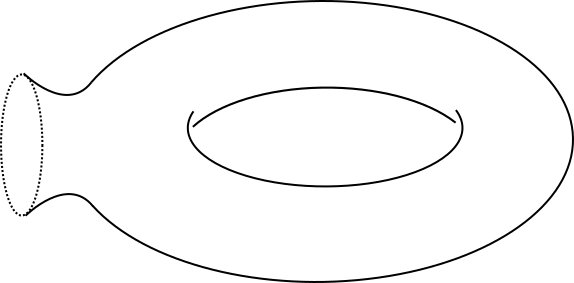
\includegraphics[width=0.5\textwidth]{handle.png}
\caption{A handle.}
\end{figure}

\begin{prop}\label{surface-loops} Let $\Sigma$ be a surface of genus $g$. There exist finite families $R=\{r_i\}$ and $B=\{b_j\}$ of loops on $\Sigma$ such that:
\begin{enumerate}
\item Two loops in the same family are disjoint.
\item Any point of the surface belongs to at most two loops.
\item The loops divide the surface into a disjoint family of regions, each of them a disk (up to homeomorphism).
\end{enumerate}
\end{prop}

\begin{proof} We give an explicit construction of such families.

The case in which $g=0$ (the sphere) is easily dealt with by choosing a single loop $r_1$ as the equator, since both hemispheres are homeomorphic to a disk and the other conditions are vacuously true.

For the cases in which $g>0$, we will make use of the handle decomposition we mentioned previously. We will draw a handle as a square (with opposite edges identified) having a gray hole in its center. Consider the following configuration:

\begin{figure}[h]
\[
\begin{tikzpicture}
\draw (0,0) node[minimum size=6cm,draw] {};

\fill [black,opacity=.15] circle (2cm);

\draw[red] (-3,1) -- (-1.73,1);
\draw[red] (-3,-1) -- (-1.73,-1);

\draw[red] (3,1) -- (1.73,1);
\draw[red] (3,-1) -- (1.73,-1);

\draw[red] (1,-3) -- (1,-1.73);
\draw[red] (-1,-3) -- (-1,-1.73);

\draw[red] (1,3) -- (1,1.73);
\draw[red] (-1,3) -- (-1,1.73);

\draw[blue] (0,0) circle (2cm);
\end{tikzpicture}
\]
\end{figure}

We first deal with the case in which $g=1$. If we glue such a handle to the boundary of the following disk, we obtain a torus with a single red loop $r_1$ and a single blue loop $b_1$:

\begin{figure}[h]
\label{divided-handle}
\[
\begin{tikzpicture}

\draw[red] (-2.83,1) to [bend right=50] (-1,2.83);
\draw[red] (2.83,1) to [bend left=50] (1,2.83);
\draw[red] (2.83,-1) to [bend right=50] (1,-2.83);
\draw[red] (-2.83,-1) to [bend left=50] (-1,-2.83);

\draw[blue] (0,0) circle (3cm);
\end{tikzpicture}
\]
\end{figure}

Once again, the intersection conditions are vacuous. Finally, we observe that the blue loop cuts the torus into a disk and a handle, so one can check condition $3$ in both objects separately. One sees at once that the disk gets cut up into 5 smaller disks, while the handle is divided into $3$ disks, as we wanted.

\marginpar{a lo largo de esta seccion todas las refs a lemas están mal}

While the solution to the case $g=1$ may be easier to draw directly on a square instead of considering a handle decomposition, the latter helps to illustrate the general case, which we now consider. For the case $g>1$, we regard our surface as a disk with $g-1$ holes, with a handle divided as in \ref{divided-handle} attached to its boundary and to each of its holes. We now exemplify the configuration on the \textcolor{red}{holed} disk for $g=4$:

\begin{figure}[h]
\[
\begin{tikzpicture}
\draw[red] (-5.44, 0.5) -- (-3.87, 0.5);
\draw[red] (-5.44, -0.5) -- (-3.87, -0.5);
\draw[red] (5.44, 0.5) -- (3.87, 0.5);
\draw[red] (5.44, -0.5) -- (3.87, -0.5);

\draw[red] (-3.5,0.87) -- (-3.5,2.7);
\draw[red] (-3.5,-0.87) -- (-3.5,-2.7);
\draw[red] (3.5,0.87) -- (3.5,2.7);
\draw[red] (3.5,-0.87) -- (3.5,-2.7);

\draw[red] (-2.137, 0.5) -- (-0.863, 0.5);
\draw[red] (-2.137, -0.5) -- (-0.863, -0.5);
\draw[red] (2.137, 0.5) -- (0.863, 0.5);
\draw[red] (2.137, -0.5) -- (0.863, -0.5);

\draw[red] (-2.5,0.87) to [bend left=40] (-0.5,0.87);
\draw[red] (2.5,0.87) to [bend right=40] (0.5,0.87);
\draw[red] (-2.5,-0.87) to [bend right=40] (-0.5,-0.87);
\draw[red] (2.5,-0.87) to [bend left=40] (0.5,-0.87);

\draw[blue] (0,0) ellipse (5.5cm and 3.5cm);
\draw[blue] (0,0) circle (1cm);
\draw[blue] (-3,0) circle (1cm);
\draw[blue] (3,0) circle (1cm);
\fill [black,opacity=.15] (-3,0) circle (1cm);
\fill [black,opacity=.15] (0,0) circle (1cm);
\fill [black,opacity=.15] (3,0) circle (1cm);
\end{tikzpicture}
\]
\end{figure}

The following is an outline for the construction of the previous figure for general $g$:
\begin{enumerate}
\item Place the $g-1$ holes in a straight line inside the disk.
\item Connect the boundary of the left and rightmost holes to the boundary of the disk using 4 red arcs, mimicking the figure.
\item Cycle through the holes from left to right. If the current hole has a neighboring hole to its right, draw 4 red arcs connecting their boundaries.
\end{enumerate}

Notice that after gluing the handles, both the red and the blue arcs are now loops. We now consider the families $\{r_i\}$ and $\{b_j\}$, consisting of the red and blue loops respectively. Inspecting the figures, we see that conditions 1 and 2 are both satisfied. Finally, it remains to check condition 3. Since we have already seen that each handle is split up into disks in the discussion of the case $g=1$, it suffices to check this for the \textcolor{red}{holed} disk, and once again this is easily seen from the drawing.
\end{proof}


A \emph{band} on a surface $\Sigma$ is a finite sequence $\{C_1, \dots, C_n\}$, where each $S_i$ is a quadrilateral on $\Sigma$ subdivided by one of its main diagonals, arranged as in one of the following two figures:

\[
\begin{tikzpicture}
\draw (-5,1) -- (5,1);
\draw (-5,-1) -- (5,-1);

\foreach \x in {-4,-2,...,4}
\draw (\x,1) -- (\x,-1);

\foreach \x in {-4,-2,...,2}
\draw (\x,-1) -- (\x+2, 1);

\node at (-5,-1.4) {$\dots$};
\node at (-3,-1.4) {$C_{n-1}$};
\node at (-1,-1.4) {$C_{n}$};
\node at (1,-1.4) {$C_{1}$};
\node at (3,-1.4) {$C_{2}$};
\node at (5,-1.4) {$\dots$};
\end{tikzpicture}
\]

\[
\begin{tikzpicture}
\draw (-5,1) -- (5,1);
\draw (-5,-1) -- (5,-1);

\foreach \x in {-4,-2,...,4}
\draw (\x,1) -- (\x,-1);

\foreach \x in {-4,-2,...,2}
\draw (\x,1) -- (\x+2, -1);

\node at (-5,-1.4) {$\dots$};
\node at (-3,-1.4) {$C_{n-1}$};
\node at (-1,-1.4) {$C_{n}$};
\node at (1,-1.4) {$C_{1}$};
\node at (3,-1.4) {$C_{2}$};
\node at (5,-1.4) {$\dots$};
\end{tikzpicture}
\]

Notice that in both cases the choice of diagonal is consistent throughout the band. We will say a band is \emph{positively oriented} if it is arranged as in the first figure and \emph{negatively oriented} otherwise. We require that the only adjacency relations between quadrilaterals in a band are the ones expressed by the figures, so in particular bands have well-defined top and bottom sides. We remark that two differently oriented bands may intersect as the following figure shows:

\[
\label{band-intersection}
\begin{tikzpicture}
\draw (-4,-1) -- (4,-1);
\draw (-4,1) -- (4,1);
\draw (-1,4) -- (-1,-4);
\draw (1,-4) -- (1,4);
\foreach \x in {-3,-1,...,3}
{
\draw (\x,-1) -- (\x, 1);
\draw (-1,\x) -- (1,\x);
}
\foreach \x in {-3,-1,1}
{
\draw (\x,-1) -- (\x+2,1);
\draw (-1,\x) -- (1,\x+2);
}
\end{tikzpicture}
\]

Given a surface $\Sigma$ of arbitrary genus, we consider families of loops $R=\{r_i\}$ and $B=\{b_j\}$ on $\Sigma$ satisfying the conditions stated in proposition \ref{surface-loops}. We can now pick suitably small tubular neighborhoods of each loop and place a positively (resp. negatively) oriented band over each neighborhood corresponding to a loop in $R$ (resp. $B$). Conditions 1 and 2 of proposition \ref{surface-loops} guarantee that all intersections between bands resemble that of figure \ref{band-intersection}. Condition 3 guarantees that each connected component of the complement of the bands is a polygon. We will refer to these polygons as \emph{regions}. Therefore, the collection of bands and regions actually define a polygonal subdivision of $\Sigma$. \textcolor{red}{For technical reasons that will be clearer later, we will require each band to have at least 5 quadrilaterals between any pair of intersections with other bands. This can be easily achieved by refining the division of the band if necessary.} We will refer to this hypothesis as $(\diamond)$ throughout this section. From now on we fix a subdivision as described above for each genus $g$ and call its associated QP $(Q_g,P_g)$. The corresponding Jacobian algebra will be denoted $A_g$.

\begin{figure}[h]
\[
\begin{tikzpicture}
%aristas
\draw (-5, .75) -- (5, .75);
\draw (-5, -.75) -- (5, -.75);
\draw (-5, -5.25) -- (5, -5.25);
\draw (-5, -6.75) -- (5, -6.75);
\draw (-2.25, -8.25) -- (-2.25, 2.25);
\draw (-3.75, -8.25) -- (-3.75, 2.25);
\draw (2.25, -8.25) -- (2.25, 2.25);
\draw (3.75, -8.25) -- (3.75, 2.25);

\foreach \x in {-3.75,-2.25,...,3.75}
{
\draw (\x, .75) -- (\x, -.75);
\draw (\x, -5.25) -- (\x, -6.75);
}

\foreach \x in {-6.75,-5.25,...,1.75}
{
\draw (-3.75, \x) -- (-2.25, \x);
\draw (3.75, \x) -- (2.25, \x);
}

\foreach \x in {-3.75,-2.25,...,2.25}
{
\draw (\x, -.75) -- (\x+1.5, .75);
\draw (\x, -6.75) -- (\x+1.5, -5.25);
}

\foreach \x in {-6.75,-5.25,...,0.25}
{
\draw (-3.75, \x) -- (-2.25, \x+1.5);
\draw (3.75, \x+1.5) -- (2.25, \x);
}

%flechas del quiver
\foreach \x in {-3.75,-2.25,...,2.25}
{
\draw[->, red] (\x+0.85, -0.65) -- (\x+1.4, -0.05);
\draw[->, red] (\x+1.4, 0) -- (\x+0.85, 0);
\draw[->, red] (\x+0.75, -0.1) -- (\x+0.75, -0.65);
\draw[->, red] (\x+0.85, -6.65) -- (\x+1.4, -6.05);
\draw[->, red] (\x+1.4, -6) -- (\x+0.85, -6);
\draw[->, red] (\x+0.75, -6.1) -- (\x+0.75, -6.65);

\draw[->, red] (\x+0.75, 0.1) -- (\x+0.75, 0.65);
\draw[->, red] (\x+0.65, 0.65) -- (\x+0.1, 0.1);
\draw[->, red] (\x+0.1, 0) -- (\x+0.65, 0);
\draw[->, red] (\x+0.75, -5.9) -- (\x+0.75, -5.35);
\draw[->, red] (\x+0.65, -5.35) -- (\x+0.1, -5.9);
\draw[->, red] (\x+0.1, -6) -- (\x+0.65, -6);
}

\foreach \x in {-0.75,-2.25,-3.75}
{
\draw[->, red] (-2.35, \x-0.75) -- (-2.9, \x-0.75);
\draw[->, red] (-3, \x-0.85) -- (-3, \x-1.4);
\draw[->, red] (-2.9, \x-1.4) -- (-2.35, \x-0.85);
\draw[->, red] (3.65, \x-0.75) -- (3.1, \x-0.75);
\draw[->, red] (3, \x-0.85) -- (3, \x-1.4);
\draw[->, red] (3.1, \x-1.4) -- (3.65, \x-0.85);

\draw[->, red] (-3, \x-0.65) -- (-3, \x-0.1);
\draw[->, red] (-3.1, \x-0.1) -- (-3.65, \x-0.65);
\draw[->, red] (-3.65, \x-0.75) -- (-3.1, \x-0.75);
\draw[->, red] (3, \x-0.65) -- (3, \x-0.1);
\draw[->, red] (2.9, \x-0.1) -- (2.35, \x-0.65);
\draw[->, red] (2.35, \x-0.75) -- (2.9, \x-0.75);
}

\draw[<-, red] (-1.4, -0.85) to [bend right] (-0.1, -0.85);
\draw[<-, red] (0.1, -0.85) to [bend right] (1.4, -0.85);
\draw[->,  red] (-1.4, -5.15) to [bend left] (-0.1, -5.15);
\draw[->, red] (0.1, -5.15) to [bend left] (1.4, -5.15);

\draw[->, red] (-2.15, -1.65) to [bend left] (-2.15, -2.9);
\draw[->, red] (-2.15, -3.1) to [bend left] (-2.15, -4.35);
\draw[<-, red] (2.15, -1.65) to [bend right] (2.15, -2.9);
\draw[<-, red] (2.15, -3.1) to [bend right] (2.15, -4.35);

\draw[->, red] (-1.6, -0.85) to [bend left] (-2.15, -1.45);
\draw[->, red] (-2.15, -4.55) to [bend left] (-1.6, -5.15);
\draw[<-, red] (1.6, -0.85) to [bend right] (2.15, -1.45);
\draw[<-, red] (2.15, -4.55) to [bend right] (1.6, -5.15);
\end{tikzpicture}
\]
\caption{The configuration of the associated quiver $Q_g$ around a region.}
\end{figure}
We now turn to the study of some relations that hold in $A_g$, that will enable us to prove its finite-dimensionality.

\begin{lemma}\label{band-sides} Any path in $A_g$ passing through vertices of both sides of a band is zero.
\end{lemma}
\begin{proof} Throughout this and the following proofs, we will only consider our bands to be positively oriented, since the analogous statements for negatively oriented bands are proved in a similar fashion. We name the arrows in the quiver as in the following figure:

\[
\begin{tikzpicture}[text width=1.5mm, font=\footnotesize]
\draw (-5, 0) -- (5, 0);
\draw (-5, 2) -- (5, 2);
\foreach \x in {-3,-1,...,3}
\draw (\x, 0) -- (\x, 2);
\foreach \x in {-3,-1,1}
{
\draw (\x,0) -- (\x+2, 2);
\draw [->, red] (\x+1.9, 1) to node[above] {$b$} (\x+1.1, 1);
\draw[->, red] (\x+1, 0.9) to node[left]{$f$} (\x+1, 0.1);
\draw[->, red] (\x+1.1, 0.1) to node[right]{$a$} (\x+1.9, 0.9);
\draw[->, red] (\x+1, 1.1) to node[right]{$c$} (\x+1, 1.9);
\draw[->, red] (\x+0.9, 1.9) to node[left]{$d$} (\x+0.1, 1.1);
\draw[->, red] (\x+0.1, 1) to node[below]{$e$} (\x+0.9, 1);
}

\draw[->, red, dashed] (-1.9, 2.1) to [bend left] node[above]{$x$} (-0.1, 2.1);
\draw[->, red, dashed] (0.1, 2.1) to [bend left] node[above]{$x$} (2.1, 2.1);
\draw[<-, red, dashed] (-1.9, -0.1) to [bend right] node[below]{$y$} (-0.1, -0.1);
\draw[<-, red, dashed] (0.1, -0.1) to [bend right] node[below]{$y$} (2.1, -0.1);
\end{tikzpicture}
\]

Since our quiver arises from a polygonal subdivision, we know that there is a cycle around each vertex,\marginpar{esto hay que probarlo en algún momento} and so each $x$ and each $y$ are paths of length at least 1. We mark those paths in the figure with a dashed arrow. We have given the same name to arrows occupying the same position in different squares, since this abuse of notation will be useful for calculation.

Inspecting the figure we see that any path passing through vertices of both sides of the band must contain a path of the form $cba$ or $fed$ as factors. It suffices to check that both of them are zero in $A_g$.

We have that $\partial_f(P_g) = ba + eay$, and so $ba  = -eay$ in $A_g$. Therefore, we have that $cba = -ceay$. Moreover, $\partial_d(P_g) = ce + xcb$, from which we deduce that $ce = -xcb$ in $A_g$. Putting all of this together, we get that $cba=-ceay=xcbay$ (one should note that the $cba$ factor in the right hand side of the equality consists of arrows placed on the square immediately left from the one where we started). Proceeding inductively we get $cba=x^ncbay^n$ for all positive $n$. Since $x$ and $y$ are paths of length at least $1$, this shows that $cba$ is equal to paths of arbitrarily high length. Therefore, we conclude that $cba=0$ in $A_g$. \marginpar{esto también hay que hacerlo...}

An analogous argument shows that $fed=0$ in $A_g$ as well, concluding the proof. 
\end{proof}

\begin{lemma}\label{long-band-paths} Any sufficiently long path contained entirely in bands is zero in $A_g$. More precisely, any non-zero path contained in a single band (resp. several bands) is of length at most 5 (resp. 9).
\end{lemma}
\begin{proof} We first prove that any sufficiently long path cotained entirely in a single band is zero. As we have already seen, any path passing through vertices of both sides of the band is zero, so we will suppose without loss of generality that our path is placed on the upper part of the band. Mantaining the notation used on the proof of the previous lemma, this is equivalent to saying our path only has arrows $b, c, d$ or $e$ as factors.

We start by studying paths containing a $3$-cycle as a prefix. The $3$-cycles $edc$ and $ced$ only prefix two paths of length 4, namely $cedc$ and $dced$. Since $\partial_e(P_g) = dc + ayf$, the relation $dc = -ayf$ holds, and so $cedc=-ceayf=0$ and $dced=-ayfed=0$ by lemma \ref{band-sides}. Moreover, the $3$-cycle $dce$ only prefixes two paths of length 5, which are $cbdce$ and $cedce$. Clearly, $cedce=0$ since we have already shown that $cedc=0$, and using the relation $dc=-ayf$ we get $cbdce = - cbayfe=0$ once again by lemma \ref{band-sides}.

Now we turn to paths containing a $3$-cycle as a suffix. Once again, the $3$-cycles $ced$ and $dce$ only suffix two paths of length 4, which are $cedc$ and $dced$, already shown to be zero previously. The $3$-cycle $edc$ is a suffix to only two paths of length 5, which are $edcbd$ and $edced$. We see that $edced=0$ since $dced=0$ and $edcbd=-eayfbd=0$ as we wanted.

Therefore, any path in a band of length $>5$ containing a 3-cycle is zero, since we have shown these cycles only admit prefixes and suffixes of length at most 1.

Now, a path of length $>5$ not containing a 3-cycle is either of the form $dcbdcb$, $bdcbdc$ or $cdbcbd$. All possibilites have $cbdc$ as a factor, which is clearly zero since $cbdc = -cbayf = 0$ by lemma \ref{band-sides}. Therefore, we conclude that any path of length $>5$ contained in a single band is zero.

Finally, consider a path of length $>9$ contained in possibly different bands. If its first six arrows lie on the same band, the path is zero as seen previously. Otherwise, at most five of its first arrows lie on the same band and the sixth is then placed on a different band intersecting the original one, as seen in the following figure:

\[
\begin{tikzpicture}
\draw (-3.5*1.25, 0) -- (1.5*1.25, 0);
\draw (-3.5*1.25, -1.25) -- (1.5*1.25, -1.25);
\draw (0,3.5*1.25) -- (0,-1.5*1.25);
\draw (1.25,3.5*1.25) -- (1.25,-1.5*1.25);

\foreach \x in {-3.75,-2.5,...,0}
{
\draw (\x,-1.25) -- (\x+1.25, 0);
\draw (0, -\x) -- (1.25, -\x);
\draw (\x,0) -- (\x, -1.25);
}

\foreach \x in {0,1.25,...,2.5}
\draw (0, \x) -- (1.25, \x+1.25);

\draw[->, red] (0.5*1.25, 1.5*1.25 - 0.1) -- (0.5*1.25, 1.25 + 0.1);
\draw[->, red] (0.5*1.25 - 0.1, 1.25-0.1) -- (0.1, 0.5*1.25+0.1);
\draw[->, red] (0.1, 0.5*1.25) -- (0.5*1.25 - 0.1, 0.5*1.25);
\draw[->, red] (0.5*1.25, 0.5*1.25-0.1) -- (0.5*1.25, 0.1);
\draw[->, red] (0.5*1.25 - 0.1, -0.1) -- (0.1, -0.5*1.25+0.1);
\draw[->, red] (-0.1, -0.5*1.25) -- (-0.5*1.25+0.1, -0.5*1.25);
\draw[->, red] (-0.5*1.25, -0.5*1.25+0.1) -- (-0.5*1.25, -0.1);
\draw[->, red] (-0.5*1.25 - 0.1, -0.1) -- (-1.25 + 0.1, -0.5*1.25+0.1);
\draw[->, red] (-1.25 -0.1, -0.5*1.25) -- (-1.5*1.25+0.1, -0.5*1.25);
\end{tikzpicture}
\]

Since by hypothesis $(\diamond)$ \marginpar{quizás podria haber un link a la def de $\diamond$}two intersections in the same band are distanced by at least \textcolor{red}{five} quadrilaterals, we conclude that at least the next \textcolor{red}{six} arrows belong to the same band. Therefore, any path of length $>9$ contained entirely in bands is zero in $A_g$, as we wanted.
\end{proof}

\begin{lemma}\label{long-region-paths} Any non-zero path entirely contained in an $n$-sided region is of length at most $3n-4$.
\end{lemma}
\begin{proof} We fix an $n$-sided region. Consider any band neighboring our region and pick any of its squares that is at least two squares away from an intersection with another band, which is always possible by hypothesis $(\diamond)$. Recalling the fact that our region induces an $n$-cycle in the quiver, we name the arrow starting at the square we picked as $x_0$. In general, given $j\in \ZZ/n\ZZ$ we call $x_j$ the arrow starting at the target of $x_{j-1}$. Keeping the previous notation for arrows contained in bands, our current situation is illustrated by this figure:

\[
\begin{tikzpicture}[text width=1.5mm, font=\footnotesize]
\draw (-6, 0) -- (6, 0);
\draw (-6, 2) -- (6, 2);
\foreach \x in {-5,-3,...,5}
\draw (\x, 0) -- (\x, 2);
\foreach \x in {-5,-3,...,3}
{
\draw (\x,0) -- (\x+2, 2);
\draw [->, red] (\x+1.9, 1) to node[above] {$b$} (\x+1.1, 1);
\draw[->, red] (\x+1, 0.9) to node[left]{$f$} (\x+1, 0.1);
\draw[->, red] (\x+1.1, 0.1) to node[right]{$a$} (\x+1.9, 0.9);
\draw[->, red] (\x+1, 1.1) to node[right]{$c$} (\x+1, 1.9);
\draw[->, red] (\x+0.9, 1.9) to node[left]{$d$} (\x+0.1, 1.1);
\draw[->, red] (\x+0.1, 1) to node[below]{$e$} (\x+0.9, 1);
}

\draw[->, red, dashed] (-5+1.1, 2.1) to [bend left] node[above]{$x_{n-2}$} (-5+2.9, 2.1);
\draw[->, red, dashed] (-3+1.1, 2.1) to [bend left] node[above]{$x_{n-1}$} (-3+2.9, 2.1);
\draw[->, red, dashed] (-1+1.1, 2.1) to [bend left] node[above]{$x_{0}$} (-1+2.9, 2.1);
\draw[->, red, dashed] (1+1.1, 2.1) to [bend left] node[above]{$x_{1}$} (1+2.9, 2.1);
\end{tikzpicture}
\]

\marginpar{hay que centrar los labels del dibujo}We now prove that the path $L=x_{n-1}x_{n-2}\dots x_2x_1x_{0}x_{n-1}\dots x_3x_2$ is zero. We have that $\partial_{x_0}(P_g)=x_{n-1}x_{n-2}\dots x_2x_1+cbd$ and $\partial_{x_1}(P_g)=x_{0}x_{n-1}\dots x_3x_2+cbd$. Therefore, the relations
\begin{align*}
x_{n-1}x_{n-2}\dots x_2x_1=-cbd\\
x_{0}x_{n-1}\dots x_3x_2=-cbd
\end{align*}
hold in $A_g$. We stress that $cbd$ denotes a different path in each one of the two equations: they are similar paths contained in different squares. Using this relations, we see that $$ x_{n-1}x_{n-2}\dots x_2x_1x_{0}x_{n-1}\dots x_3x_2=-cbdx_{0}x_{n-1}\dots x_3x_2=cbdcbd,$$ and the latter is zero by lemma \ref{long-band-paths} since $cbdcbd$ is a path of length 6 lying on a single band. 

Finally, since the longest path entirely contained in our region not having $L$ as a factor is
$$x_{n-2}x_{n-1}\dots x_0x_{n-1}x_{n-2}\dots x_0x_{n-1}x_{n-2}\dots x_3,$$
\marginpar{poner las longitudes con ganchitos}which is of length $3n-4$, the result follows.
\end{proof}

\begin{lemma} \label{long-br-paths} Any sufficiently long path not having factors from two different regions is zero in $A_g$.
\end{lemma}
\begin{proof} We write our path as $B_{k+1}R_k\dots R_2 B_2 R_1 B_1$, where the paths $R_i$ are contained in a same region and the paths $B_j$ are non-trivial (except possibly for $B_1$ and $B_{k+1}$) and contained in bands.

Let $1<j<k+1$. The path $B_j$ starts and ends at the boundary of our region of interest. Therefore, it must pass through both of the endpoints of a same arrow belonging to the cycle associated to the region, which we will call $x_0$ following the notation employed in the proof of lemma \label{long-band-paths}.\marginpar{esto no está particularmente claro...} Therefore, using the relation induced by $\partial_{x_0}(P_g)$, we can replace some of the arrows in $B_j$ with a path entirely contained in the region.
After applying this argument repeatedly, we can then suppose our path is of the form $B_2 R_1 B_1$. The proof now follows from lemmas \ref{long-band-paths} and \ref{long-region-paths}, since if our path is non-zero, then $|B_1|<10$, $|B_2|<10$ and $|R_1|<3n-3$, where $n$ is the number of sides of the region.
\end{proof}

After proving all these lemmas, the main result of this section now easily follows:

\begin{thm} The algebra $A_g$ is finite-dimensional.
\end{thm}
\begin{proof} By lemma \ref{long-br-paths}, any sufficiently long path is zero if it does not have factors from two different regions, but any path that does must be zero (regardless of length) by lemma \ref{band-sides}, since it must cross a band. Therefore, any sufficiently long path is zero, and so $A_g$ is finite-dimensional.
\end{proof}
\end{section}
\end{chapter}
\begin{bibdiv}
\begin{biblist}[\normalsize]
%\bib{AM69}{book}{
%   author={Atiyah, M. F.},
%  author={Macdonald, I. G.},
%   title={Introduction to commutative algebra},
%   publisher={Addison-Wesley Publishing Co., Reading, Mass.-London-Don
%   Mills, Ont.},
%   date={1969},
%   pages={ix+128},
%   review={\MR{0242802 (39 \#4129)}},
%}

\bib{Ber78}{article}{
   author={Bergman, George M.},
   title={The diamond lemma for ring theory},
   journal={Adv. in Math.},
   volume={29},
   date={1978},
   number={2},
   pages={178--218},
   issn={0001-8708},
   review={\MR{506890 (81b:16001)}},
   doi={10.1016/0001-8708(78)90010-5},
}

%\bib{Bou98}{book}{
%   author={Bourbaki, Nicolas},
%   title={Commutative algebra. Chapters 1--7},
%   series={Elements of Mathematics (Berlin)},
%   note={Translated from the French;
%   Reprint of the 1989 English translation},
%   publisher={Springer-Verlag, Berlin},
%   date={1998},
%   pages={xxiv+625},
%   isbn={3-540-64239-0},
%   review={\MR{1727221 (2001g:13001)}},
%}

\bib{DWZ08}{article}{
   author={Derksen, Harm},
   author={Weyman, Jerzy},
   author={Zelevinsky, Andrei},
   title={Quivers with potentials and their representations. I. Mutations},
   journal={Selecta Math. (N.S.)},
   volume={14},
   date={2008},
   number={1},
   pages={59--119},
   issn={1022-1824},
   review={\MR{2480710 (2010b:16021)}},
   doi={10.1007/s00029-008-0057-9},
}

\bib{FFG93}{article}{
   author={Farkas, Daniel R.},
   author={Feustel, C. D.},
   author={Green, Edward L.},
   title={Synergy in the theories of Gr\"obner bases and path algebras},
   journal={Canad. J. Math.},
   volume={45},
   date={1993},
   number={4},
   pages={727--739},
   issn={0008-414X},
   review={\MR{1227656 (94d:13030)}},
   doi={10.4153/CJM-1993-041-8},
}

\bib{FST08}{article}{
   author={Fomin, Sergey},
   author={Shapiro, Michael},
   author={Thurston, Dylan},
   title={Cluster algebras and triangulated surfaces. I. Cluster complexes},
   journal={Acta Math.},
   volume={201},
   date={2008},
   number={1},
   pages={83--146},
   issn={0001-5962},
   review={\MR{2448067 (2010b:57032)}},
   doi={10.1007/s11511-008-0030-7},
}

\bib{Hel02}{thesis}{
   author={Hellström, Lars},
   title={The diamond lemma for power series algebras},
   school={Umeå University, Department of Mathematics},
   date={2002},
   eprint={http://urn.kb.se/resolve?urn=urn:nbn:se:umu:diva-92}
}

\bib{LF09}{article}{
   author={Labardini-Fragoso, Daniel},
   title={Quivers with potentials associated to triangulated surfaces},
   journal={Proc. Lond. Math. Soc. (3)},
   volume={98},
   date={2009},
   number={3},
   pages={797--839},
   issn={0024-6115},
   review={\MR{2500873 (2010b:16033)}},
   doi={10.1112/plms/pdn051},
}

\bib{Lad12}{article}{
   author={Ladkani, Sefi},
   title={On Jacobian algebras from closed surfaces},
   date={2012},
   eprint={arXiv:1207.3778 [math.RT]}
}

\bib{Mas77}{book}{
   author={Massey, William S.},
   title={Algebraic topology: an introduction},
   note={Reprint of the 1967 edition;
   Graduate Texts in Mathematics, Vol. 56},
   publisher={Springer-Verlag, New York-Heidelberg},
   date={1977},
   pages={xxi+261 pp. ISBN 0-387-90271-6},
   review={\MR{0448331 (56 \#6638)}},
}

\bib{Red01}{article}{
   author={Redondo, Mar{\'{\i}}a Julia},
   title={Hochschild cohomology: some methods for computations},
   note={IX Algebra Meeting USP/UNICAMP/UNESP (Portuguese) (São
   Pedro, 2001)},
   journal={Resenhas},
   volume={5},
   date={2001},
   number={2},
   pages={113--137},
   issn={0104-3854},
   review={\MR{1945297 (2004a:16015)}},
}

\bib{RSS80}{article}{
   author={Rota, Gian-Carlo},
   author={Sagan, Bruce},
   author={Stein, Paul R.},
   title={A cyclic derivative in noncommutative algebra},
   journal={J. Algebra},
   volume={64},
   date={1980},
   number={1},
   pages={54--75},
   issn={0021-8693},
   review={\MR{575782 (82b:05017)}},
   doi={10.1016/0021-8693(80)90133-7},
}

\bib{SAV15}{article}{
   author={Suárez-Alvarez, Mariano},
   author={Vivas, Quimey},
   title={\textcolor{red}{PONER TITULO DEL PREPRINT}},
   date={2015}
}

\bib{Sti82}{article}{
   author={Stillwell, John},
   title={The word problem and the isomorphism problem for groups},
   journal={Bull. Amer. Math. Soc. (N.S.)},
   volume={6},
   date={1982},
   number={1},
   pages={33--56},
   issn={0273-0979},
   review={\MR{634433}},
   doi={10.1090/S0273-0979-1982-14963-1},
}

\bib{TVD12}{article}{
   author={Trepode, Sonia},
   author={Valdivieso-Díaz, Yadira}
   title={On finite dimensional Jacobian Algebras},
   date={2012},
   eprint={arXiv:1207.1917v4 [math.RT]}
}

\bib{VD14}{thesis}{
   author={Valdivieso-Díaz, Yadira},
   title={Sobre álgebras Jacobianas de dimensión finita},
   school={Universidad Nacional de Mar del Plata},
   date={2014}
}

\bib{Wei94}{book}{
   author={Weibel, Charles A.},
   title={An introduction to homological algebra},
   series={Cambridge Studies in Advanced Mathematics},
   volume={38},
   publisher={Cambridge University Press, Cambridge},
   date={1994},
   pages={xiv+450},
   isbn={0-521-43500-5},
   isbn={0-521-55987-1},
   review={\MR{1269324 (95f:18001)}},
   doi={10.1017/CBO9781139644136},
}
\end{biblist}
\end{bibdiv}


\end{document}